\section{Summary}

Fixed points and (known) conserved quantites for the non-concentric (NCAP) families in this chapter appear in
\cref{tab:04-n3-non-conc-families} (compare with 
\cref{tab:03-n3-conc-families}).

A diagram depicting how certain pairs of families are interrelated by either similarity or polar transformations appears in in \cref{fig:04-transformations}.

\begin{table}
\centering
\begin{tabular}{|r|c|c|l|}
\hline
Family & Fixed & Conserves & Notes \\
\hline
\makecell[rc]{Poristic\\(bicentric)} & $X_1$, $X_3$, $X_{40}$, $\ldots$ & $\sum\cos\theta_i,a_9/b_9$ & \makecell[lc]{polar image of Confocal family\\wrt to a focus} \\
\hline
\makecell[rt]{Poristic\\Excentrals} & $X_2$, $X_3$, $X_4$, $X_5$ & $\sum{s_i^2}$, $\prod\cos\theta_i$ & \makecell[lt]{Inscribed in circle;\\caustic is MacBeath inconic} \\
\hline
Brocard & \makecell[lc]{$X_3$, $X_6$, $X_{15}$, $X_{16}$,\\$X_{39}$, $X_{182},\ldots$,\\$\Omega_1$, $\Omega_2$} & $\sum{s_i^{-2}}$, $\omega$, $\sum\cot\theta_i$ & \makecell[lc]{polar image of Homothetic\\family wrt caustic focus;\\inscribed in circle;\\caustic is Brocard inellipse}\\
%\hline
%focus-Inversive & $X_7$ & $L,\sum\cos\theta_i$ & \makecell[lc]{inversive image of Confocals\\wrt a focus; non-Ponceletian;\\inscribed in Pascal's limaçon;\\caustic non-ellipse}\\
\hline
\end{tabular}
\caption{Summary of fixed points and (known) conserved quantites for the non-concentric, axis-parallel (NCAP) families in this chapter.}
\label{tab:04-n3-non-conc-families}
\end{table}

% \includegraphics[trim={left bot right top},clip]
\begin{figure}
    \centering
    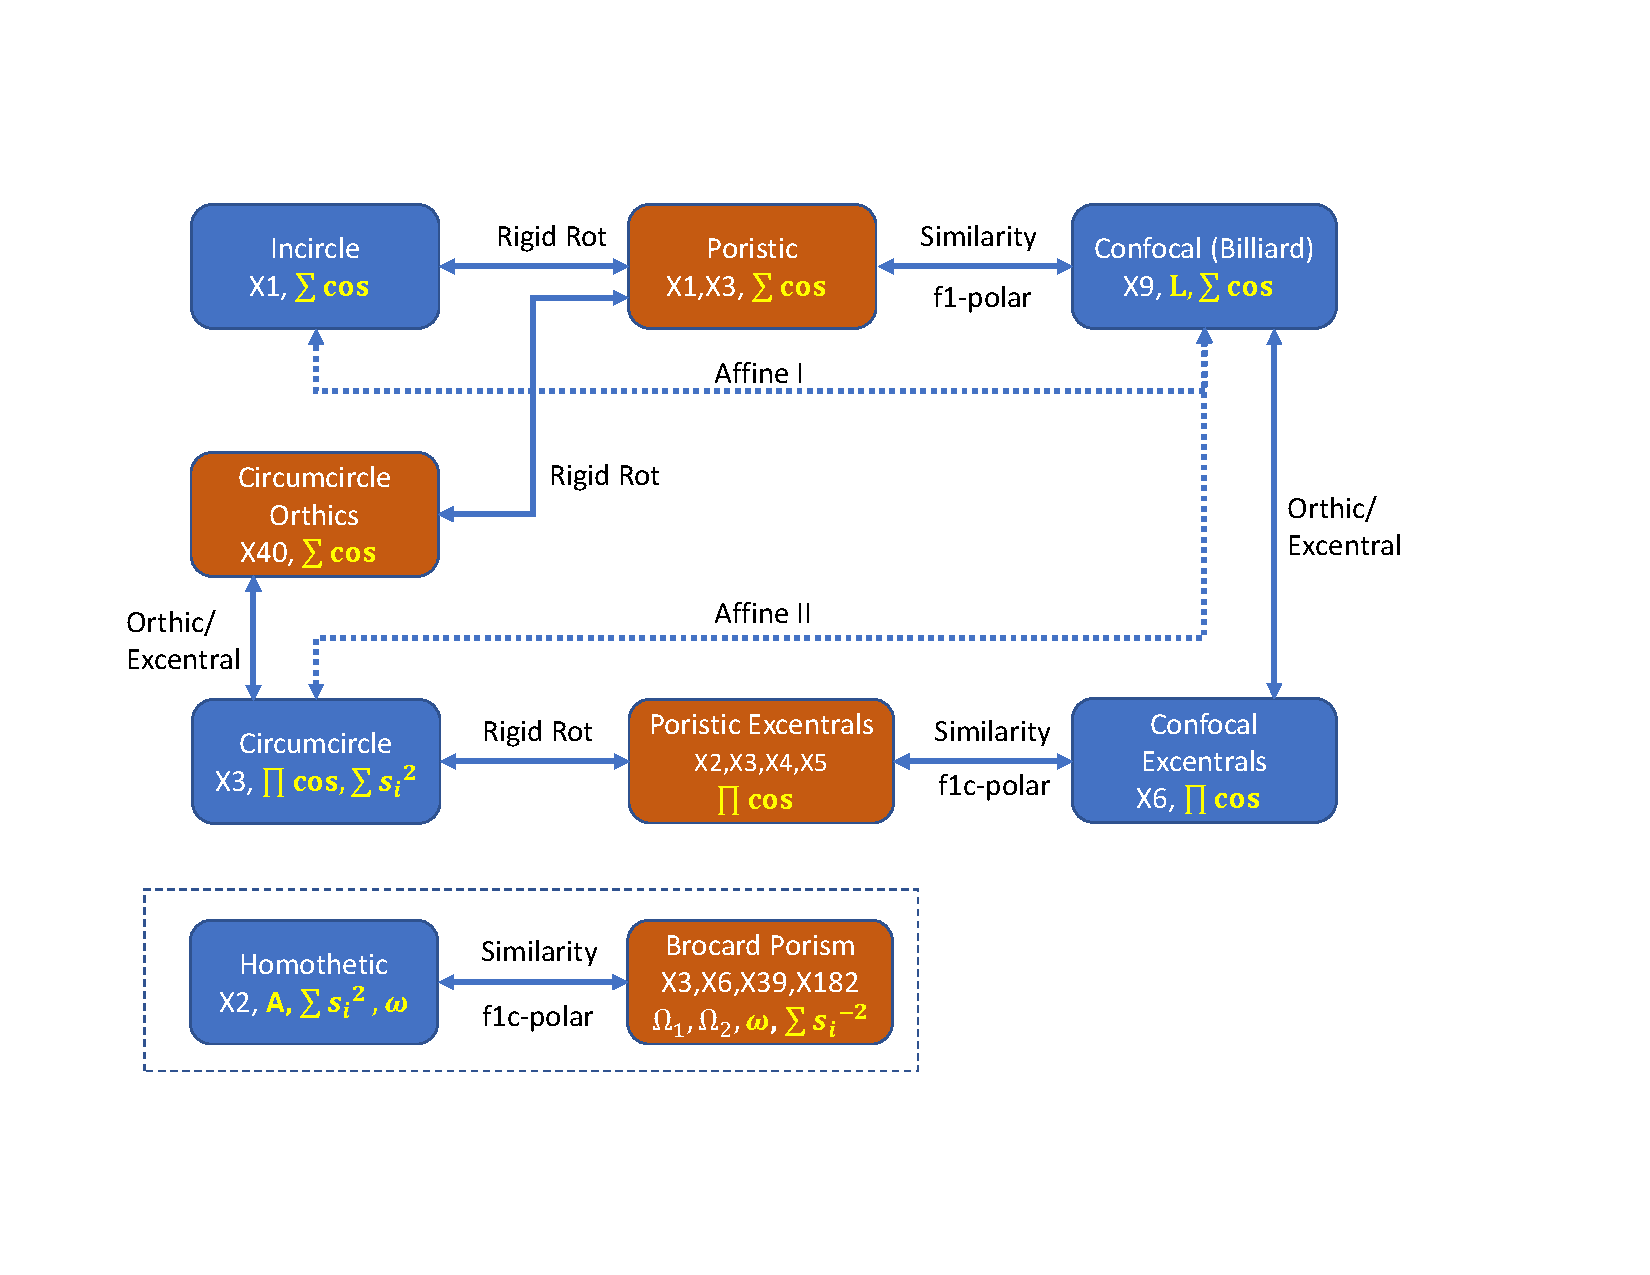
\includegraphics[trim={60 90 80 90},clip,width=\textwidth]{pics_04_250_poncelet_transformations.pdf}
  \caption{Families mentioned in this chapter (blue ones are concentric, tan ones are non-concentric), as well as the transformations under which certain families are interrelated.}
    \label{fig:04-transformations}
\end{figure}